\documentclass[notes]{beamer}

\usepackage[T1]{fontenc}
\usepackage[utf8]{inputenc}
\usepackage[polish]{babel}

\usepackage{minted}
\usepackage{pifont}
\usepackage{listings}
\usepackage{pgfplots}
\usepackage{xcolor}

\usepackage[sfdefault]{FiraSans}

\usetheme{default}
\usecolortheme{seahorse}
\useoutertheme{default}
\useinnertheme{default}
\setbeamertemplate{section in toc}[square]
%\setbeamertemplate{section in toc}[sections numbered]
\setbeamertemplate{navigation symbols}{}
\setbeamerfont{frametitle}{size=\LARGE}

\definecolor{lightgrey}{gray}{0.95}
\setbeamercolor{block title}{bg=lightgrey}
\setbeamercolor{block body}{bg=lightgrey}

\linespread{1.2}

\newcommand\Header[1]{%
  \begin{frame}
  \vfill
  \centering
  \begin{beamercolorbox}[sep=8pt,center]{title}
    \usebeamerfont{title}#1\par%
  \end{beamercolorbox}
  \vfill
  \end{frame}
}

\AtBeginSection[]{\Header{\insertsectionhead}}

\newcommand\Wider[2][3em]{%
\makebox[\linewidth][c]{%
  \begin{minipage}{\dimexpr\textwidth+#1\relax}
  \raggedright#2
  \end{minipage}%
  }%
}

\graphicspath{{prez-img/}}

\newcommand{\createhist}[3]{
  \begin{tikzpicture}[font=\tiny, trim axis left, trim axis right]
    \begin{axis}[ybar, ymin=0, xticklabel={$\pgfmathprintnumber{\tick}$ ms}, #3]
      \addplot +[hist={data=x, bins=50}, opacity=0.5, draw=none, red] table [y index=0] {#1};
      \addplot +[hist={data=x, bins=50}, opacity=0.5, draw=none, blue] table [y index=0] {#2};
      \legend{
        Old -- \input|"wc -l #1 | cut -d' ' -f1" invocations,
        New -- \input|"wc -l #2 | cut -d' ' -f1" invocations
      }
    \end{axis}
  \end{tikzpicture}
}

\newcommand{\createbar}[4]{
  \begin{tikzpicture}[font=\tiny, trim axis left, trim axis right]
    \begin{axis}[
        width=#3,
        xmin=0, xmax=3, xtick={1,2},
        x tick style={draw=none},
        xticklabels={Old,New},
        ymin=0,
        nodes near coords,
        every axis plot/.append style={
          ybar,
          bar width=#4cm,
          bar shift=0pt,
          fill,
          text opacity=1, fill opacity=0.5, 
        }
    ]
      \addplot[draw=none, fill=red] coordinates {(1, #1)};
      \addplot[draw=none, fill=blue] coordinates {(2, #2)};
    \end{axis}
  \end{tikzpicture}
}

\title{Efektywny mechanizm copy-on-write\\dla systemu operacyjnego Mimiker}
\author{Franciszek Zdobylak}
\institute{Instytut Informatyki\\Uniwersytet Wrocławski}
\date{22 marca 2024}

\begin{document}
\maketitle

\begin{frame}{Spis treści}
  \vfill
  \tableofcontents
  \vfill
\end{frame}

\section{Pamięć wirtualna}

\begin{frame}{Pamięć fizyczna}
  \vfill
  \textbf{\large Budowa}
  \vfill
  \begin{itemize}
    \item Główna pamięć -- RAM
      \begin{itemize}
        \item Jednolita
        \item Dostęp z wykorzystaniem adresów (fizycznych)
      \end{itemize}
    \vfill
    \item Urządzenia pamięci
      \begin{itemize}
        \item Dyski, Pamięć flash itp.
      \end{itemize}
    \vfill
    \item Inne urządzenia
      \begin{itemize}
        \item Karta graficzna, karta dźwiękowa itp.
      \end{itemize}
  \end{itemize}
  \vfill
\end{frame}

\begin{frame}{Pamięć wirtualna}
  \onslide<1->
  {\large Warstwa abstrakcji nad pamięcią fizyczną.}
  \vfill
  \textbf{Zadania:}
  \vspace{1em}
  \begin{enumerate}
    \item<2-> Zapewnienie bezpieczeństwa
      \begin{itemize}
        \item izolacja i kontrola dostępu
      \end{itemize}
      \vspace{1em}
    \item<3-> Efektywne wykorzystanie pamięci RAM
      \vspace{1em}
    \item<4-> Uproszczenie widoku pamięci przez procesy
      \begin{itemize}
        \item iluzja posiadania całej pamięci dla siebie
      \end{itemize}
  \end{enumerate}
\end{frame}

\Header{Mechanizmy pamięci wirtualnej}

\begin{frame}{Adresy fizyczne vs wirtualne}
  \framesubtitle{Izolacja przestrzeni adresowych}
  \centering
  \includegraphics<1>[width=0.8\textwidth]{Memory-privacy.pdf}%
  \includegraphics<2>[width=0.8\textwidth]{Memory-privacy-access.pdf}%
  \includegraphics<3>[width=0.8\textwidth]{Memory-privacy-bad-access.pdf}%
  \includegraphics<4>[width=0.8\textwidth]{Memory-privacy-address-spaces.pdf}%
\end{frame}

\begin{frame}{Adresy fizyczne vs wirtualne}
  \framesubtitle{Efektywne wykorzystanie pamięci}
  \centering
  \includegraphics<1>[width=0.8\textwidth]{Fragmentation.pdf}%
  \includegraphics<2>[width=0.8\textwidth]{Fragmentation-solved.pdf}%
\end{frame}

% Mały komentarz o segmentach
\begin{frame}{Jednakowy widok pamięci}
  \centering
  \includegraphics[width=0.8\textwidth]{Segmentation-access-rights.pdf}%
\end{frame}

% Tak na prawdę wszystko dzieje się on page level
\begin{frame}{Stronicowanie}
  \centering
  \includegraphics<1>[width=0.8\textwidth]{Paging.pdf}%
  \includegraphics<2>[width=0.8\textwidth]{Paging-translation.pdf}%
\end{frame}
\begin{frame}{Wymiana stron}
  \centering
  \includegraphics<1>[width=0.8\textwidth]{Paging-page-out.pdf}%
  \includegraphics<2>[width=0.8\textwidth]{Paging-page-in.pdf}%
\end{frame}

\begin{frame}{Współdzielenie pamięci}
  \centering
  \includegraphics<1>[width=0.8\textwidth]{Memory-sharing-before.pdf}%
  \includegraphics<2>[width=0.8\textwidth]{Memory-sharing-after.pdf}%
  \includegraphics<3>[width=0.8\textwidth]{Memory-sharing-before.pdf}%
  \includegraphics<4>[width=0.8\textwidth]{Memory-sharing-ipc.pdf}%
\end{frame}

\begin{frame}{Mechanizm copy-on-write {\tt (CoW)}}

  Optymalizacja wywołania {\tt fork}.

  \vfill

  \onslide<2->
  Fork bez CoW:
  \begin{itemize}
    \item Kopiuje całą przestrzeń adresową
    \item Rodzic oraz dziecko posiadają prywatne kopie pamięci
  \end{itemize}

  \vfill

  \onslide<3->
  Fork + CoW:
  \begin{itemize}
    \item Nie kopiuje pamięci
    \item Oznacza pamięć jako "CoW"
    \item Kopiuje pojedyncze strony przy pierwszym zapisie
  \end{itemize}

\end{frame}

\begin{frame}{Standardowy {\tt fork}}
  \centering
  \includegraphics<1>[width=0.8\textwidth]{Fork-after.pdf}%
\end{frame}

\begin{frame}{\tt fork + CoW}
  \centering
  \includegraphics<1>[width=0.8\textwidth]{Fork-cow1.pdf}%
  \includegraphics<2>[width=0.8\textwidth]{Fork-cow-erased-writes.pdf}%
\end{frame}

\begin{frame}{Copy-on-write {\large \tt (dostępy do pamięci)}}
  \centering
  \includegraphics<1>[width=0.8\textwidth]{CoW-access-read-ok.pdf}%
\end{frame}

\begin{frame}{Copy-on-write {\large \tt (page fault)}}
  \centering
  \includegraphics<1>[width=0.8\textwidth]{CoW-access-write-fail.pdf}%
\end{frame}

\begin{frame}{Copy-on-write {\large \tt (kopia)}}
  \centering
  \includegraphics<1>[width=0.8\textwidth]{CoW-copy-page.pdf}%
\end{frame}
\begin{frame}{Copy-on-write {\large \tt (zapisy do pamięci)}}
  \centering
  \includegraphics<1>[width=0.8\textwidth]{CoW-access-write-ok.pdf}%
  \includegraphics<2>[width=0.8\textwidth]{CoW-access-write-fail2.pdf}%
  \includegraphics<3>[width=0.8\textwidth]{CoW-access-write-ok2.pdf}%
\end{frame}

\section{Pamięć wirtualna w systemie NetBSD (oraz~Mimikerze)}

\begin{frame}{Mapa pamięci procesu}
  \centering
  \includegraphics<1>[width=\textwidth]{VM-map-empty.pdf}%
  \includegraphics<2>[width=\textwidth]{VM-map-entries.pdf}%
  \includegraphics<3>[width=\textwidth]{VM-map-full.pdf}%
\end{frame}

\begin{frame}{Rodzaje pamięci dostępnej w systemie}%
  \onslide<2->

  {\bf Pamięć pochodząca z zasobów systemu:}
  \vspace{1em}
  \begin{itemize}
    \item Pliki mapowane w pamięć
  \end{itemize}
  \vfill

  \onslide<3->

  {\bf Pamięć anonimowa:}
  \vspace{1em}
  \begin{itemize}
    \item Pamięć przydzielona procesowi
    \item Wypełniana prywatnymi danymi procesu
    \item Niszczona gdy przestaje być używana
  \end{itemize}
\end{frame}

\begin{frame}{Struktury do opisu pamięci}
  Struktury używane w systemie NetBSD\\
  -- w systemie pamięci wirtualnej UVM.
  \vfill
  \begin{columns}[t]
    \begin{column}{5cm}
      {\bf Pamięć zasobów}

      {UVM object}

      \vfill
      \begin{figure}
        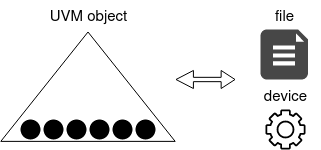
\includegraphics[width=0.8\textwidth]{UVM-object.png}
      \end{figure}
    \end{column}
    \begin{column}{5cm}
      {\bf Pamięć anonimowa}

      {Amap + Anon}

      \vfill
      \begin{figure}
        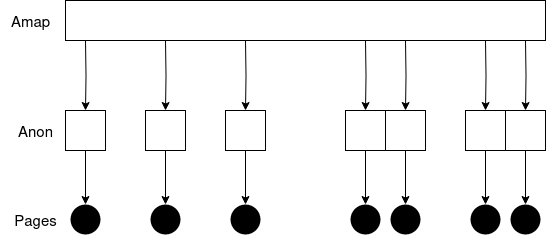
\includegraphics[width=\textwidth]{Amap.png}
      \end{figure}
    \end{column}
  \end{columns}
\end{frame}

\begin{frame}{Przykładowa mapa pamięci procesu}
  \centering
  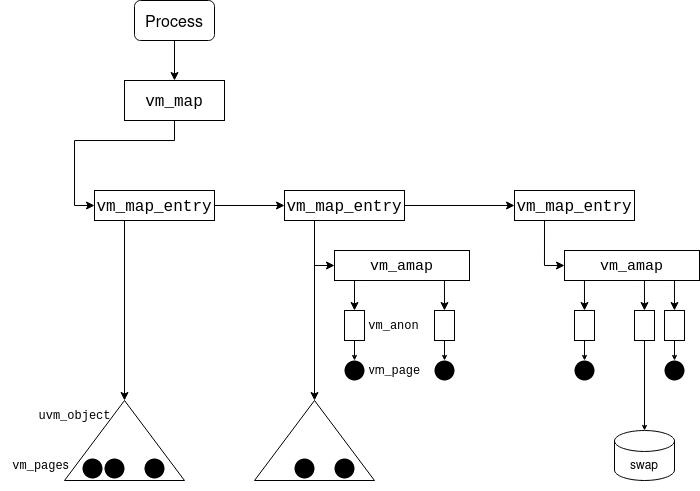
\includegraphics[width=\textwidth]{Typical-map.pdf}
\end{frame}

\section{Implementacja CoW w Mimikerze}

\begin{frame}{Zmiany}
  \linespread{1.5}
  \begin{enumerate}
    \item<1-> Zmiana implementacji podsystemu pamięci wirtualnej
      \begin{itemize}
        \item BSD VM -> UVM
        \item łatwiejszy do rozszerzania o nowe mechanizmy
      \end{itemize}
    \vfill
    \item<2-> Zaimplementowanie mechanizmu copy-on-write
    \vfill
    \item<3-> Narzędzie do analizy wydajności jądra
      \begin{itemize}
        \item Kernel Function Trace
      \end{itemize}
  \end{enumerate}
\end{frame}

\begin{frame}{Ważna  obserwacja}
  \centering
  \vspace{1cm}
  {\huge W Mimikerze występuje tylko pamięć anonimowa.}

  \vspace{2cm}

  \begin{itemize}
    \item Nie ma plików mapowanych w pamięć
    \item Nie funkcjonuje wymiana stron
  \end{itemize}

  \onslide<2->
  \begin{tikzpicture}[remember picture,overlay]
    \node at (current page.center) {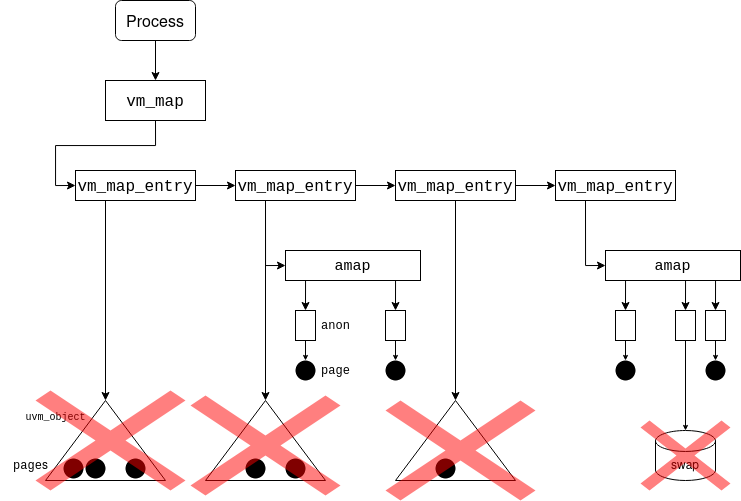
\includegraphics[width=0.95\textwidth]{Typical-map-anon.pdf}};
  \end{tikzpicture}
\end{frame}

\Header{Podsumowanie analizy wydajności}

\begin{frame}{Redukcja liczby kopiowanych stron}
  \centering
  \begin{columns}
    \begin{column}[t]{5cm}
      \begin{figure}[h]
        \centering
        \createbar{9652}{700}{1.3\textwidth}{1}
        {\footnotesize Liczba kopiowań}
      \end{figure}
    \end{column}
    \begin{column}[t]{5cm}
      \begin{figure}[h]
        \centering
        \createbar{10822}{1870}{1.3\textwidth}{1}
        {\footnotesize Sumaryczna liczba użytych stron}
      \end{figure}
    \end{column}
  \end{columns}
\end{frame}

\begin{frame}{Tworzenie nowego procesu}
  \begin{figure}[h]
    \centering
    \createhist{plots/data-prez/vm_map_clone_old.data}{plots/data-prez/vm_map_clone_new.data}{xmin=0, xmax=2.2, legend style={at={(0.02,0.89)},anchor=west}}\\
    {\footnotesize Histogram czasu wywołań dla funkcji \mintinline{c}{vm_map_clone}}
  \end{figure}
\end{frame}

\begin{frame}{Spodziewane zmiany}
  \begin{figure}[h]
    \centering
    \createbar{2958}{3668}{0.8\textwidth}{1.5}\\
    Ilość page faultów
  \end{figure}
\end{frame}

\begin{frame}{Spodziewane zmiany (2)}
  \begin{figure}[h]
    \centering
    \createbar{30}{1041}{0.8\textwidth}{1.5}\\
    Zmiana praw dostępu do stron
  \end{figure}
\end{frame}

\section{Podsumowanie}

\begin{frame}{Podsumowanie wyników pracy}
  \begin{enumerate}
    \item<1-> Implementacja mechanizmu copy-on-write
      \begin{itemize}
        \item Oszczędność pamięci
      \end{itemize}
      \vspace{1em}
    \item<2-> Ulepszenie implementacji systemu pamięci wirtualnej
      \begin{itemize}
        \item Łatwiejsza do rozszerzenia o nowe funkcje
        \item Łatwiejszy do analizy
      \end{itemize}
      \vspace{1em}
    \item<3-> Narzędzie do analizy wydajności (KFT)
      \begin{itemize}
        \item Wykrywanie operacji wymagających optymalizacji
      \end{itemize}
  \end{enumerate}
  \vfill
  \onslide<4->
  Kolejne kroki:
  \begin{itemize}
    \item Implementacja urządzeń i plików mapowanych w pamięć
    \item Implementacja wymiany stron
  \end{itemize}
\end{frame}

\end{document}

% XXX: pamięć anonimowa i uvm obiekty
%\begin{frame}{Pamięć anonimowa}
%  \begin{itemize}
%    \item Pamięć tworzona "od zera"
%      \vspace{2em}
%    \item Pamięć niszczona, gdy nikt już jej nie używa
%      \begin{itemize}
%        \item Zawiera dane widoczne tylko przez aktualny proces
%      \end{itemize}
%  \end{itemize}
%  \vfill
%  \onslide<2->
%  \begin{columns}[t]
%    \begin{column}{5cm}
%      \vfill
%      Struktury opisujące pamięć anonimową
%      \begin{itemize}
%        \item \mintinline{c}{uvm_amap}
%        \item \mintinline{c}{uvm_anon}
%      \end{itemize}
%      \vfill
%    \end{column}
%    \begin{column}{5cm}
%      \vfill
%      \vspace{0.5cm}
%      \centering
%      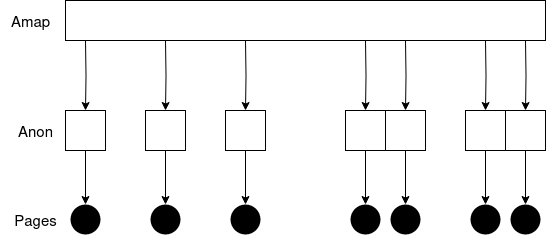
\includegraphics[width=\textwidth]{Amap.png}
%      \vfill
%    \end{column}
%  \end{columns}
%\end{frame}
%
%\begin{frame}{Pamięć pochodząca z zasobów systemu}
%  \begin{itemize}
%    \item Pliki mapowane w pamięć
%      \begin{itemize}
%          \footnotesize
%        \item Plik wykonywalny, plik z danymi
%      \end{itemize}
%    \vspace{1em}
%    \item Pamięć urządzeń
%      \begin{itemize}
%          \footnotesize
%        \item Bufory sprzętowe
%      \end{itemize}
%  \end{itemize}
%  \vfill
%  \onslide<2->
%  \begin{columns}[t]
%    \begin{column}{5cm}
%      \vfill
%      Struktury:
%      \begin{itemize}
%        \item \mintinline{c}{uvm_object}
%      \end{itemize}
%      \vfill
%    \end{column}
%    \begin{column}{5cm}
%      \vfill
%      \centering
%      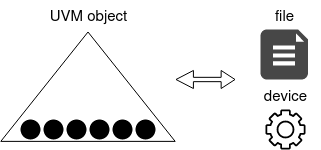
\includegraphics[width=0.8\textwidth]{UVM-object.png}
%      \vfill
%    \end{column}
%  \end{columns}
%\end{frame}

